\subsubsection{Net 4}

\zadatak Proveri kada va{\zv}i
$$
\log_{\frac{x+4}2} \left( \log_2 \frac{2x-1}{3+x} \right) < 0.
$$

\resenje
Da bi prvi logaritam bio definisan mora da va{\zv}i
$$
\frac{x+4}2>0 \land \frac{x+4}2\ne 1 \sledi
x>-4 \land x\ne -2,
$$
a kako vrednost binarnog logaritma mora biti pozitivna, onda argument mora biti
$$
\frac{2x-1}{3+x} >1\sledi x<-3 \lor x>4.
$$
Iz ovoga sledi da je funkcija je definisana pod uslovima
$$
-4<x<-3 \lor x>4.
$$

$$
\lim_{x\to \pm\infty}\left(\log_2 \frac{2x-1}{3+x}\right) =
\log_2\left(\lim_{x\to \pm\infty}\frac{2x-1}{3+x}\right) =
\log_2 2 = 1.
$$

Da bi nejednakost va{\zv}ila mora biti
\begin{align*}
    \frac{x+1}2 > 1 \land  \frac{x+1}2 > \log_2 \frac{2x-1}{3+x}  
\end{align*}

Re{\sv}e{\nj}e  je
$$
x \in \ram{(-4, -3) \cup ( 4, \infty )}.
$$
$$
\slika{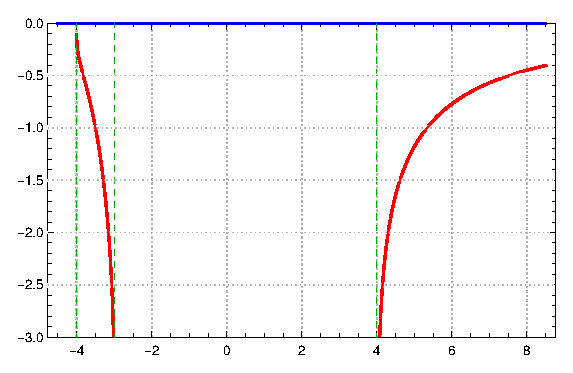
\includegraphics[width=80mm]{eps/4.eps}}{$y=\displaystyle{\log_{\frac{x+4}2} \left( \log_2 \frac{2x-1}{3+x} \right)}$.}
$$
